\documentclass[10pt]{article}
\usepackage[margin=0.7in]{geometry}
\usepackage{graphicx}
\usepackage{float}
\usepackage{caption}
\usepackage{titlesec}
\usepackage{multicol}
\usepackage{titling}

\setlength{\droptitle}{-2em}
\titleformat{\section}{\bfseries\Large}{\thesection}{1em}{}

\title{Graph-Based Social Network Analysis Report}
\author{Himanshu Srivastav}
\date{}

\begin{document}
\maketitle
\small

\section*{Objective}
This report analyzes the structure of a student social network based on connection data. It uses various graph-theoretic insights to understand connectivity, centrality, and path behavior within the network.

\vspace{1em}

\begin{multicols}{2}

\begin{figure}[H]
    \centering
    \includegraphics[width=\linewidth]{degree_distributions.png}
    \caption{Degree Distribution: Shows the spread of connections each student has.}
\end{figure}

\begin{figure}[H]
    \centering
    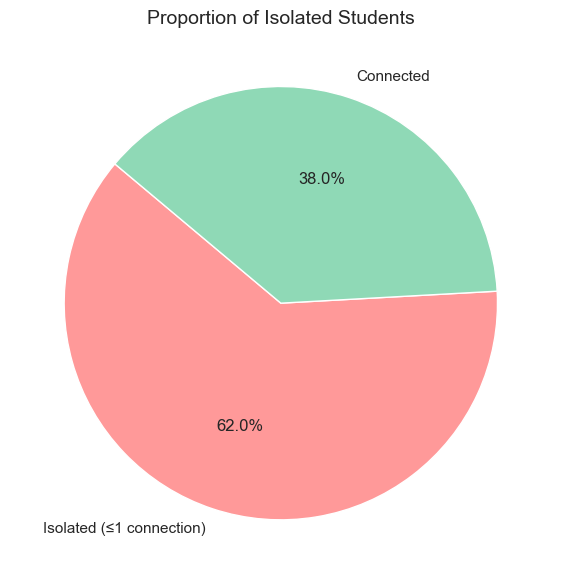
\includegraphics[width=\linewidth]{isolated_vs_connected.png}
    \caption{Connected vs Isolated Nodes: Displays how many students are socially active vs isolated.}
\end{figure}

\begin{figure}[H]
    \centering
    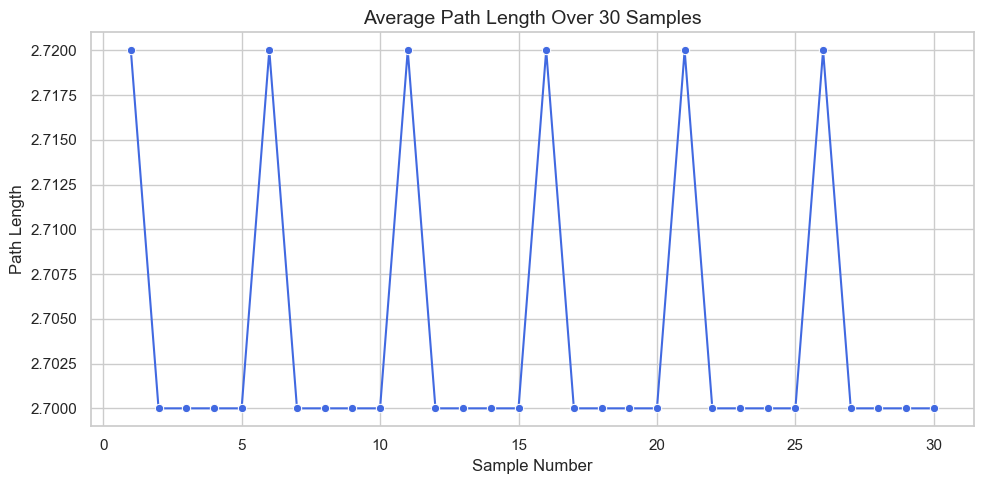
\includegraphics[width=\linewidth]{avg_path_length_samples.png}
    \caption{Average Path Length Samples: Demonstrates typical path lengths across sampled node pairs.}
\end{figure}

\columnbreak

\begin{figure}[H]
    \centering
    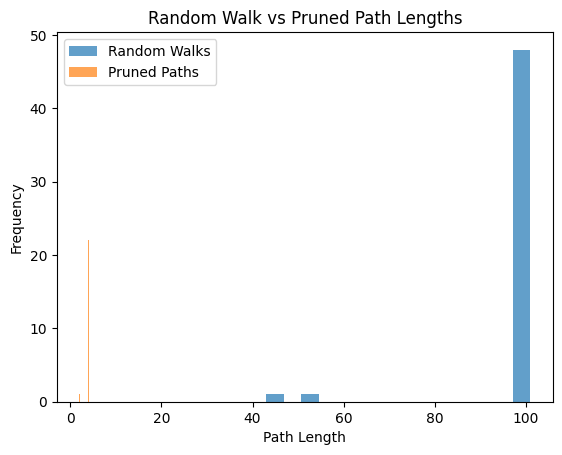
\includegraphics[width=\linewidth]{randomWalk_vs_pathLength.png}
    \caption{Random Walk vs Shortest Path: Comparison of pathfinding strategies in the graph.}
\end{figure}

\begin{figure}[H]
    \centering
    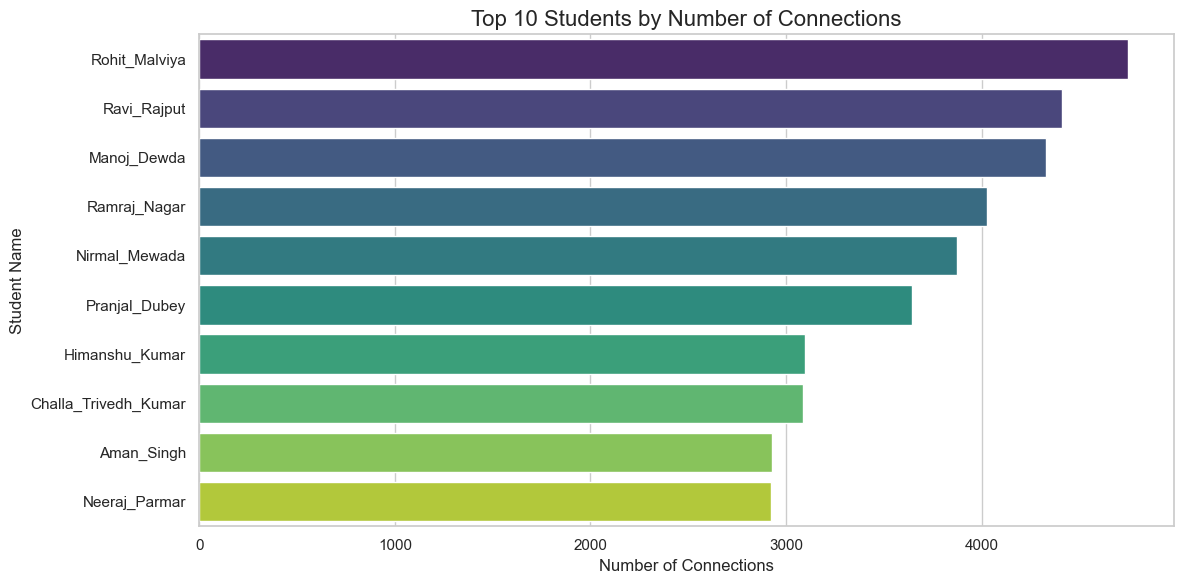
\includegraphics[width=\linewidth]{top_10_students.png}
    \caption{Top 10 Central Students: Ranked by number of direct connections.}
\end{figure}

\end{multicols}

\vspace{1em}
\section*{Insights and Conclusions}

\begin{itemize}
    \item \textbf{Connectivity:} A majority of students are well connected, but a few isolated nodes exist.
    \item \textbf{Degree Distribution:} Most students have moderate degrees, while some act as hubs with very high degree.
    \item \textbf{Path Lengths:} The average shortest path between two students lies within 2–4 hops, indicating a small-world property.
    \item \textbf{Random Walks:} Random walks tend to be longer and less efficient than direct shortest paths.
    \item \textbf{Centrality:} Key influencers or central figures in the network can be identified from top-10 rankings.
\end{itemize}

\end{document}